\documentclass[12pt]{article}

\usepackage[paperwidth=48in,paperheight=36in,margin=0.65in]{geometry}
\usepackage{graphicx}
\usepackage{xcolor}
\usepackage{multicol}
\usepackage{array}
\usepackage{booktabs}
\usepackage{hyperref}
\usepackage{url}

\pagestyle{empty}
\setlength{\parindent}{0pt}
\setlength{\parskip}{0.16in}
\setlength{\columnsep}{0.35in}
\setlength{\fboxsep}{0.22in}
\renewcommand{\arraystretch}{1.12}

\definecolor{fastnavy}{HTML}{13233A}
\definecolor{fastblue}{HTML}{2E6F9E}
\definecolor{fastgreen}{HTML}{2E8B57}
\definecolor{fastorange}{HTML}{D77A2D}
\definecolor{fastgray}{HTML}{F3F6F8}
\definecolor{fastline}{HTML}{D9E2EA}
\definecolor{fasttext}{HTML}{20252B}

\hypersetup{colorlinks=true,urlcolor=fastblue,linkcolor=fastblue}

\newcommand{\posterblock}[2]{%
  \vspace{0.12in}%
  {\color{fastnavy}\bfseries\fontsize{27}{31}\selectfont #1}\par
  \vspace{0.04in}{\color{fastline}\rule{\linewidth}{2pt}}\par
  \vspace{0.06in}#2%
}

\newcommand{\metric}[3]{%
  \fcolorbox{#1}{#1!9}{%
    \begin{minipage}[t][1.16in][c]{0.29\linewidth}
      \centering
      {\color{#1}\bfseries\fontsize{25}{28}\selectfont #2}\par
      \vspace{0.03in}
      {\fontsize{16}{19}\selectfont #3}
    \end{minipage}}%
}

\newcommand{\tightitems}{%
  \setlength{\itemsep}{0.05in}
  \setlength{\topsep}{0.03in}
  \setlength{\parsep}{0pt}
}

\begin{document}
\color{fasttext}
\fontsize{17}{20}\selectfont

{\color{fastnavy}\rule{\linewidth}{6pt}}\par
\vspace{0.10in}

\begin{minipage}[t]{0.70\linewidth}
  {\bfseries\fontsize{46}{50}\selectfont fast-tcp: Practical, Incremental Test Case Prioritization}\par
  \vspace{0.08in}
  {\color{fastblue}\bfseries\fontsize{22}{25}\selectfont Similarity-based TCP for pytest, Vitest, Go test, and JUnit/Ant workflows}
\end{minipage}
\hfill
\begin{minipage}[t]{0.27\linewidth}
  \raggedleft
  {\bfseries\fontsize{21}{24}\selectfont Tiago Lima}\par
  {\fontsize{16}{19}\selectfont Federal University of Pernambuco}\par
  {\fontsize{16}{19}\selectfont Recife, Brazil}\par
  {\fontsize{16}{19}\selectfont \texttt{tmsl@cin.ufpe.br}}
\end{minipage}

\vspace{0.18in}

\begin{center}
  \metric{fastorange}{Problem}{FAST is scalable, but adoption requires too much manual workflow glue.}
  \hspace{0.20in}
  \metric{fastblue}{Key Idea}{A Git-backed snapshot cache detects changed tests and prioritizes them first.}
  \hspace{0.20in}
  \metric{fastgreen}{Result}{0.24--0.68s absolute overhead on 576--1326 real tests.}
\end{center}

\vspace{0.02in}
\begin{multicols}{4}

\posterblock{Motivation}{
Regression suites are growing, and CI needs tests that reveal failures earlier. The FAST family of algorithms scales similarity-based test case prioritization with MinHash and locality-sensitive hashing, but earlier tooling remained hard to use in daily developer workflows.

\begin{itemize}\tightitems
  \item \textbf{Integration friction:} test representations and orchestration are often manual.
  \item \textbf{No incrementality:} unchanged tests are reprocessed every run.
  \item \textbf{Framework fragmentation:} pytest, Vitest, Go test, and JUnit need different entry points.
\end{itemize}

\fcolorbox{fastorange}{fastorange!8}{%
  \begin{minipage}{0.90\linewidth}
  {\bfseries Main question:} Can similarity-based TCP become a low-friction local tool for ordinary CI workflows?
  \end{minipage}}
}

\posterblock{Architecture}{
\begin{center}
  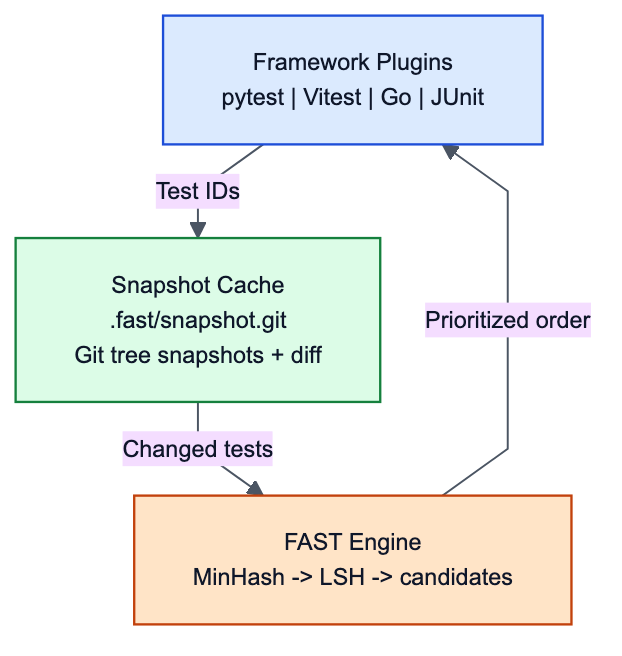
\includegraphics[width=0.88\linewidth]{figures/architecture.png}
\end{center}
\vspace{-0.06in}
\begin{itemize}\tightitems
  \item \textbf{Framework plugins} collect tests and extract black-box representations.
  \item \textbf{Snapshot cache} stores file hashes in \texttt{.fast/snapshot.git}.
  \item \textbf{FAST engine} ranks tests by dissimilarity using FAST variants.
\end{itemize}
}

\columnbreak

\posterblock{How Developers Use It}{
\fcolorbox{fastline}{fastgray}{%
  \begin{minipage}{0.91\linewidth}
  {\fontsize{15}{18}\selectfont\ttfamily
  python -m pip install -e .\\
  fast-tcp init pytest\\
  pytest --fast-tcp --fast-tcp-debug
  }
  \end{minipage}}

\vspace{0.08in}
{\fontsize{15}{18}\selectfont
\begin{tabular}{@{}lll@{}}
\toprule
Framework & Language & Mechanism \\
\midrule
pytest & Python & plugin \\
Vitest & JavaScript/TS & script helper \\
Go test & Go & script helper \\
JUnit/Ant & Java & Ant macro \\
\bottomrule
\end{tabular}}
}

\posterblock{Incremental Workflow}{
\begin{center}
  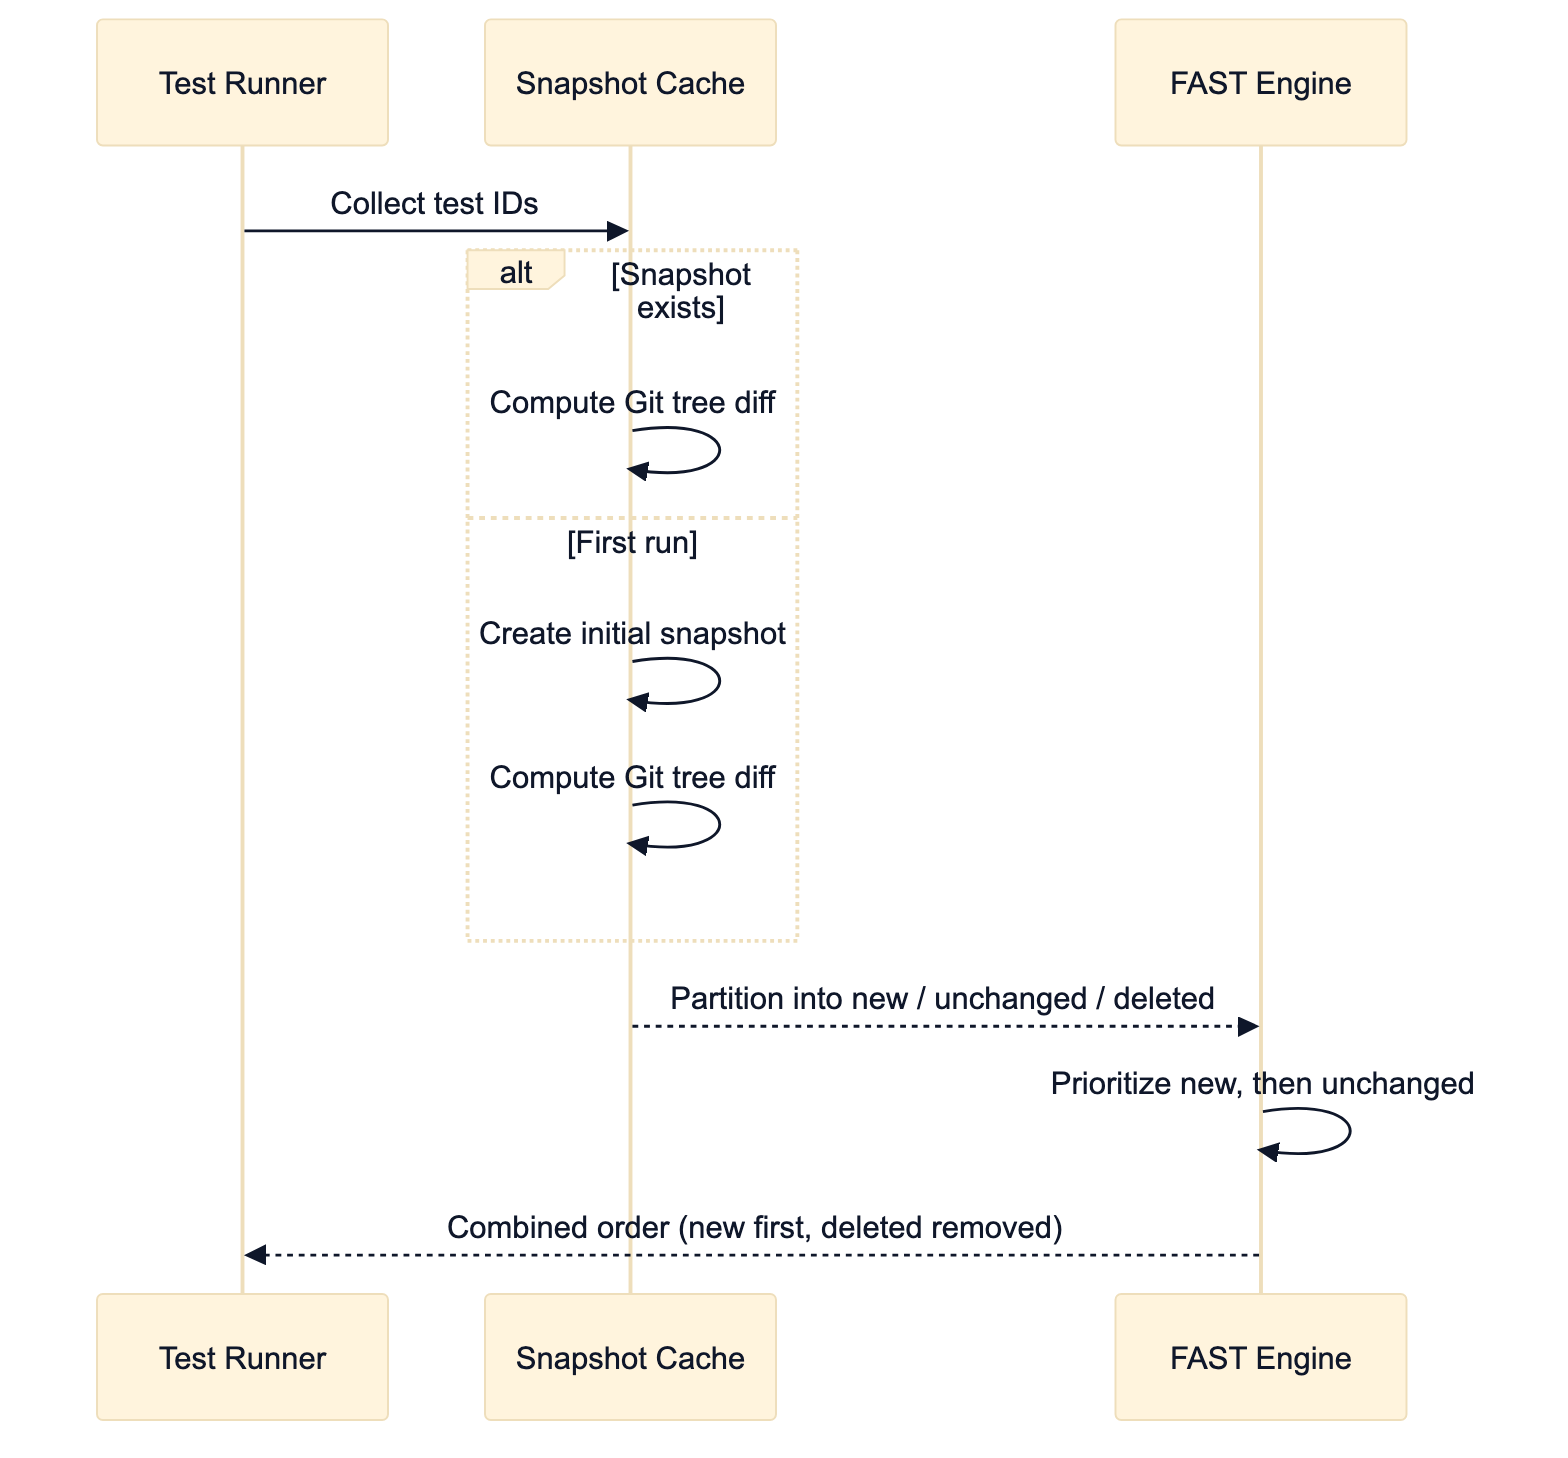
\includegraphics[width=0.95\linewidth]{figures/workflow.png}
\end{center}
\vspace{-0.08in}
\begin{enumerate}\tightitems
  \item Diff the workspace against the previous snapshot.
  \item Partition tests into new/modified, unchanged, and deleted sets.
  \item Rank new or modified tests first with FAST.
  \item Seed the cumulative signature, then rank unchanged tests.
\end{enumerate}

\fcolorbox{fastgreen}{fastgreen!8}{%
  \begin{minipage}{0.90\linewidth}
  The snapshot repository is independent of the project's own Git history, so it works with uncommitted changes and projects without useful VCS history.
  \end{minipage}}
}

\columnbreak

\posterblock{Debuggable Behavior}{
\begin{center}
  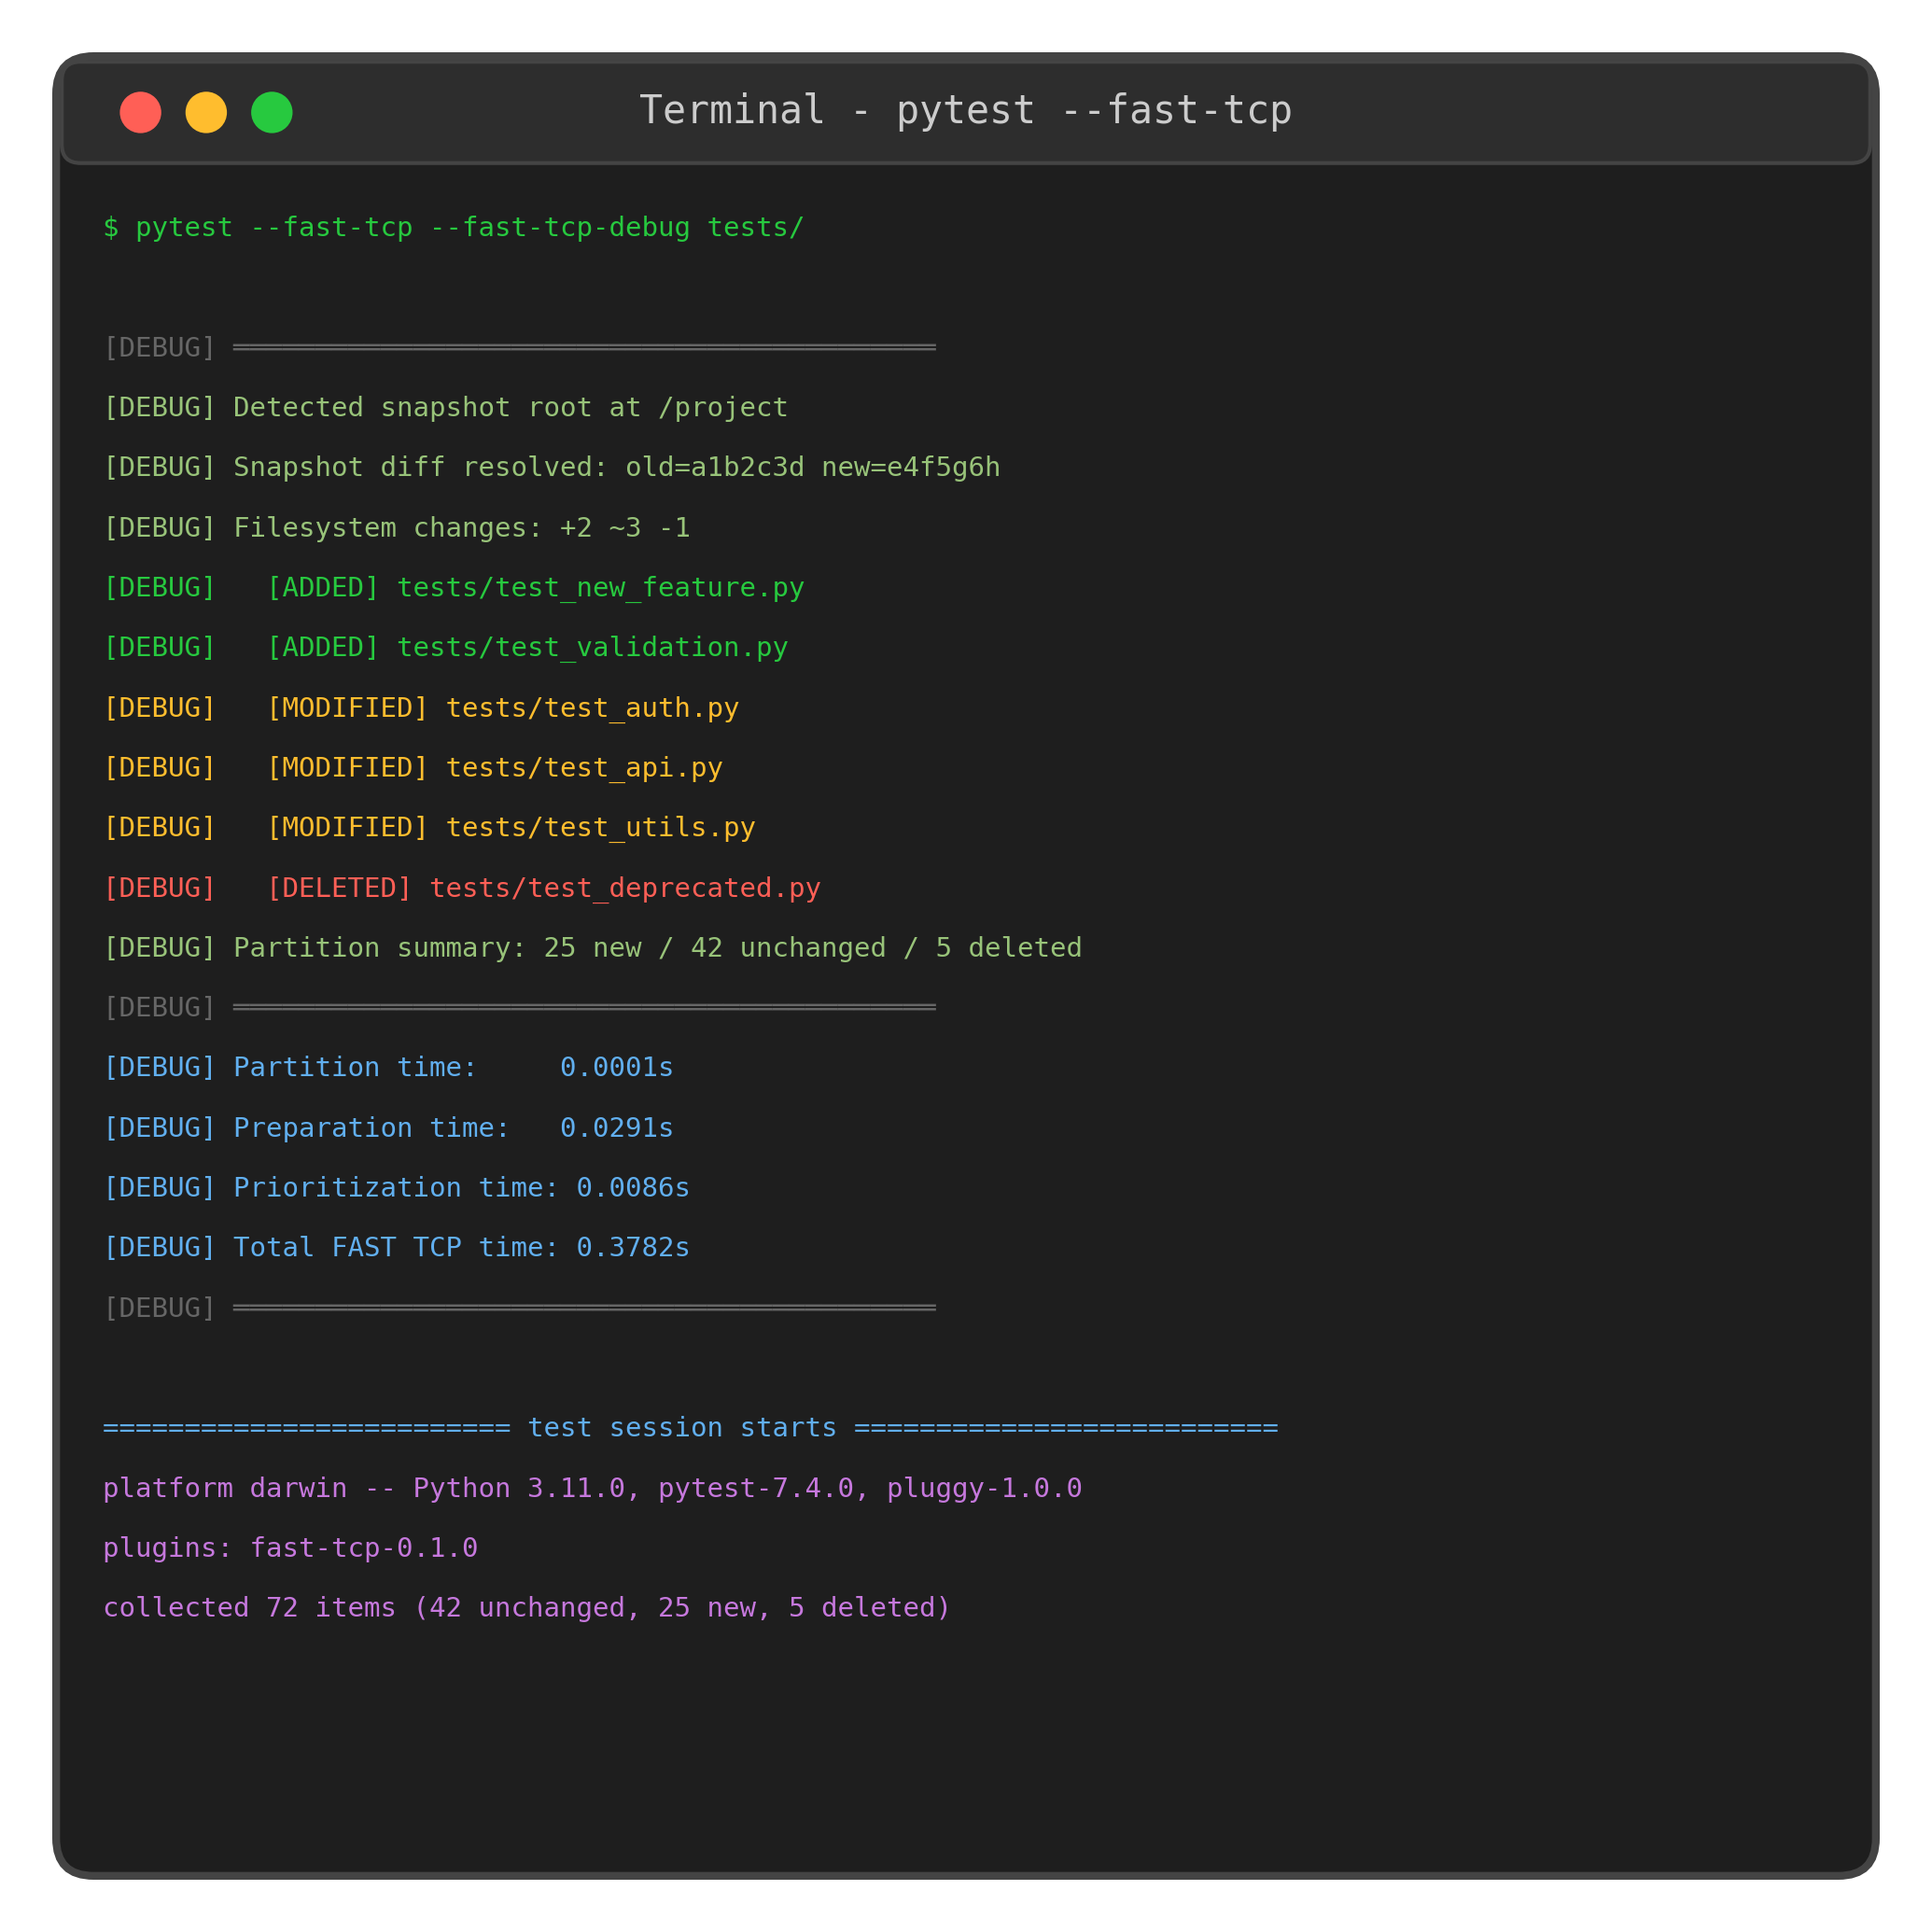
\includegraphics[width=0.78\linewidth]{figures/debug_output.png}
\end{center}
\vspace{-0.05in}
Debug output reports snapshot diff counts, test partitioning, preparation time, prioritization time, and total overhead. This makes prioritization cost visible instead of hidden inside the test runner.
}

\posterblock{Core Tradeoff}{
\begin{center}
\fcolorbox{fastblue}{fastblue!8}{%
  \begin{minipage}{0.88\linewidth}
  \centering
  {\bfseries\fontsize{25}{28}\selectfont New and modified tests first}\par
  \vspace{0.05in}
  {\fontsize{17}{20}\selectfont unchanged tests are still prioritized, but after the likely-regression surface}
  \end{minipage}}
\end{center}
\begin{itemize}\tightitems
  \item \textbf{FAST-pw:} highest search effort.
  \item \textbf{FAST-sqrt:} balanced candidate budget.
  \item \textbf{FAST-one:} lowest search effort.
\end{itemize}
}

\columnbreak

\posterblock{Real-World Evidence}{
\begin{center}
  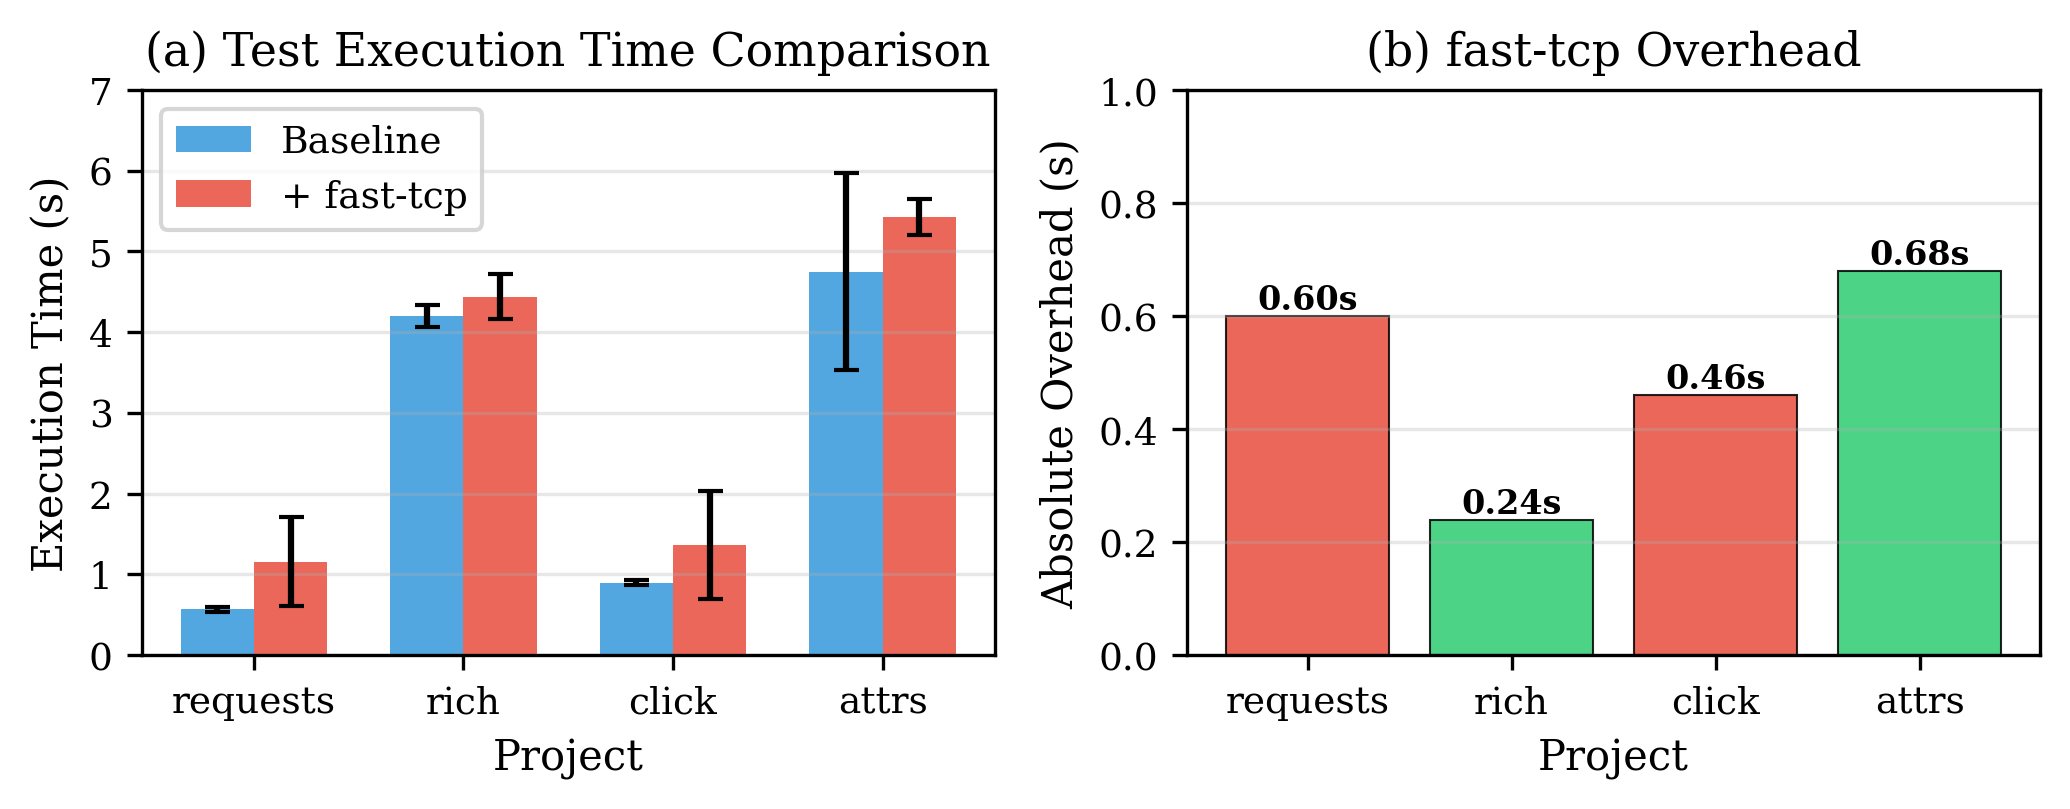
\includegraphics[width=0.92\linewidth]{figures/case_study_bar.png}
\end{center}
\vspace{-0.08in}
{\fontsize{15}{18}\selectfont
\begin{tabular}{@{}lrrrr@{}}
\toprule
Project & Tests & Baseline & Overhead & Rel. \\
\midrule
requests & 576 & 0.57s & 0.60s & 105\% \\
rich & 781 & 4.20s & 0.24s & 6\% \\
click & 611 & 0.90s & 0.46s & 51\% \\
attrs & 1326 & 4.75s & 0.68s & 14\% \\
\bottomrule
\end{tabular}}

Absolute overhead stays below one second across all projects; relative overhead drops as suite runtime grows.
}

\posterblock{Overhead Composition}{
\begin{center}
  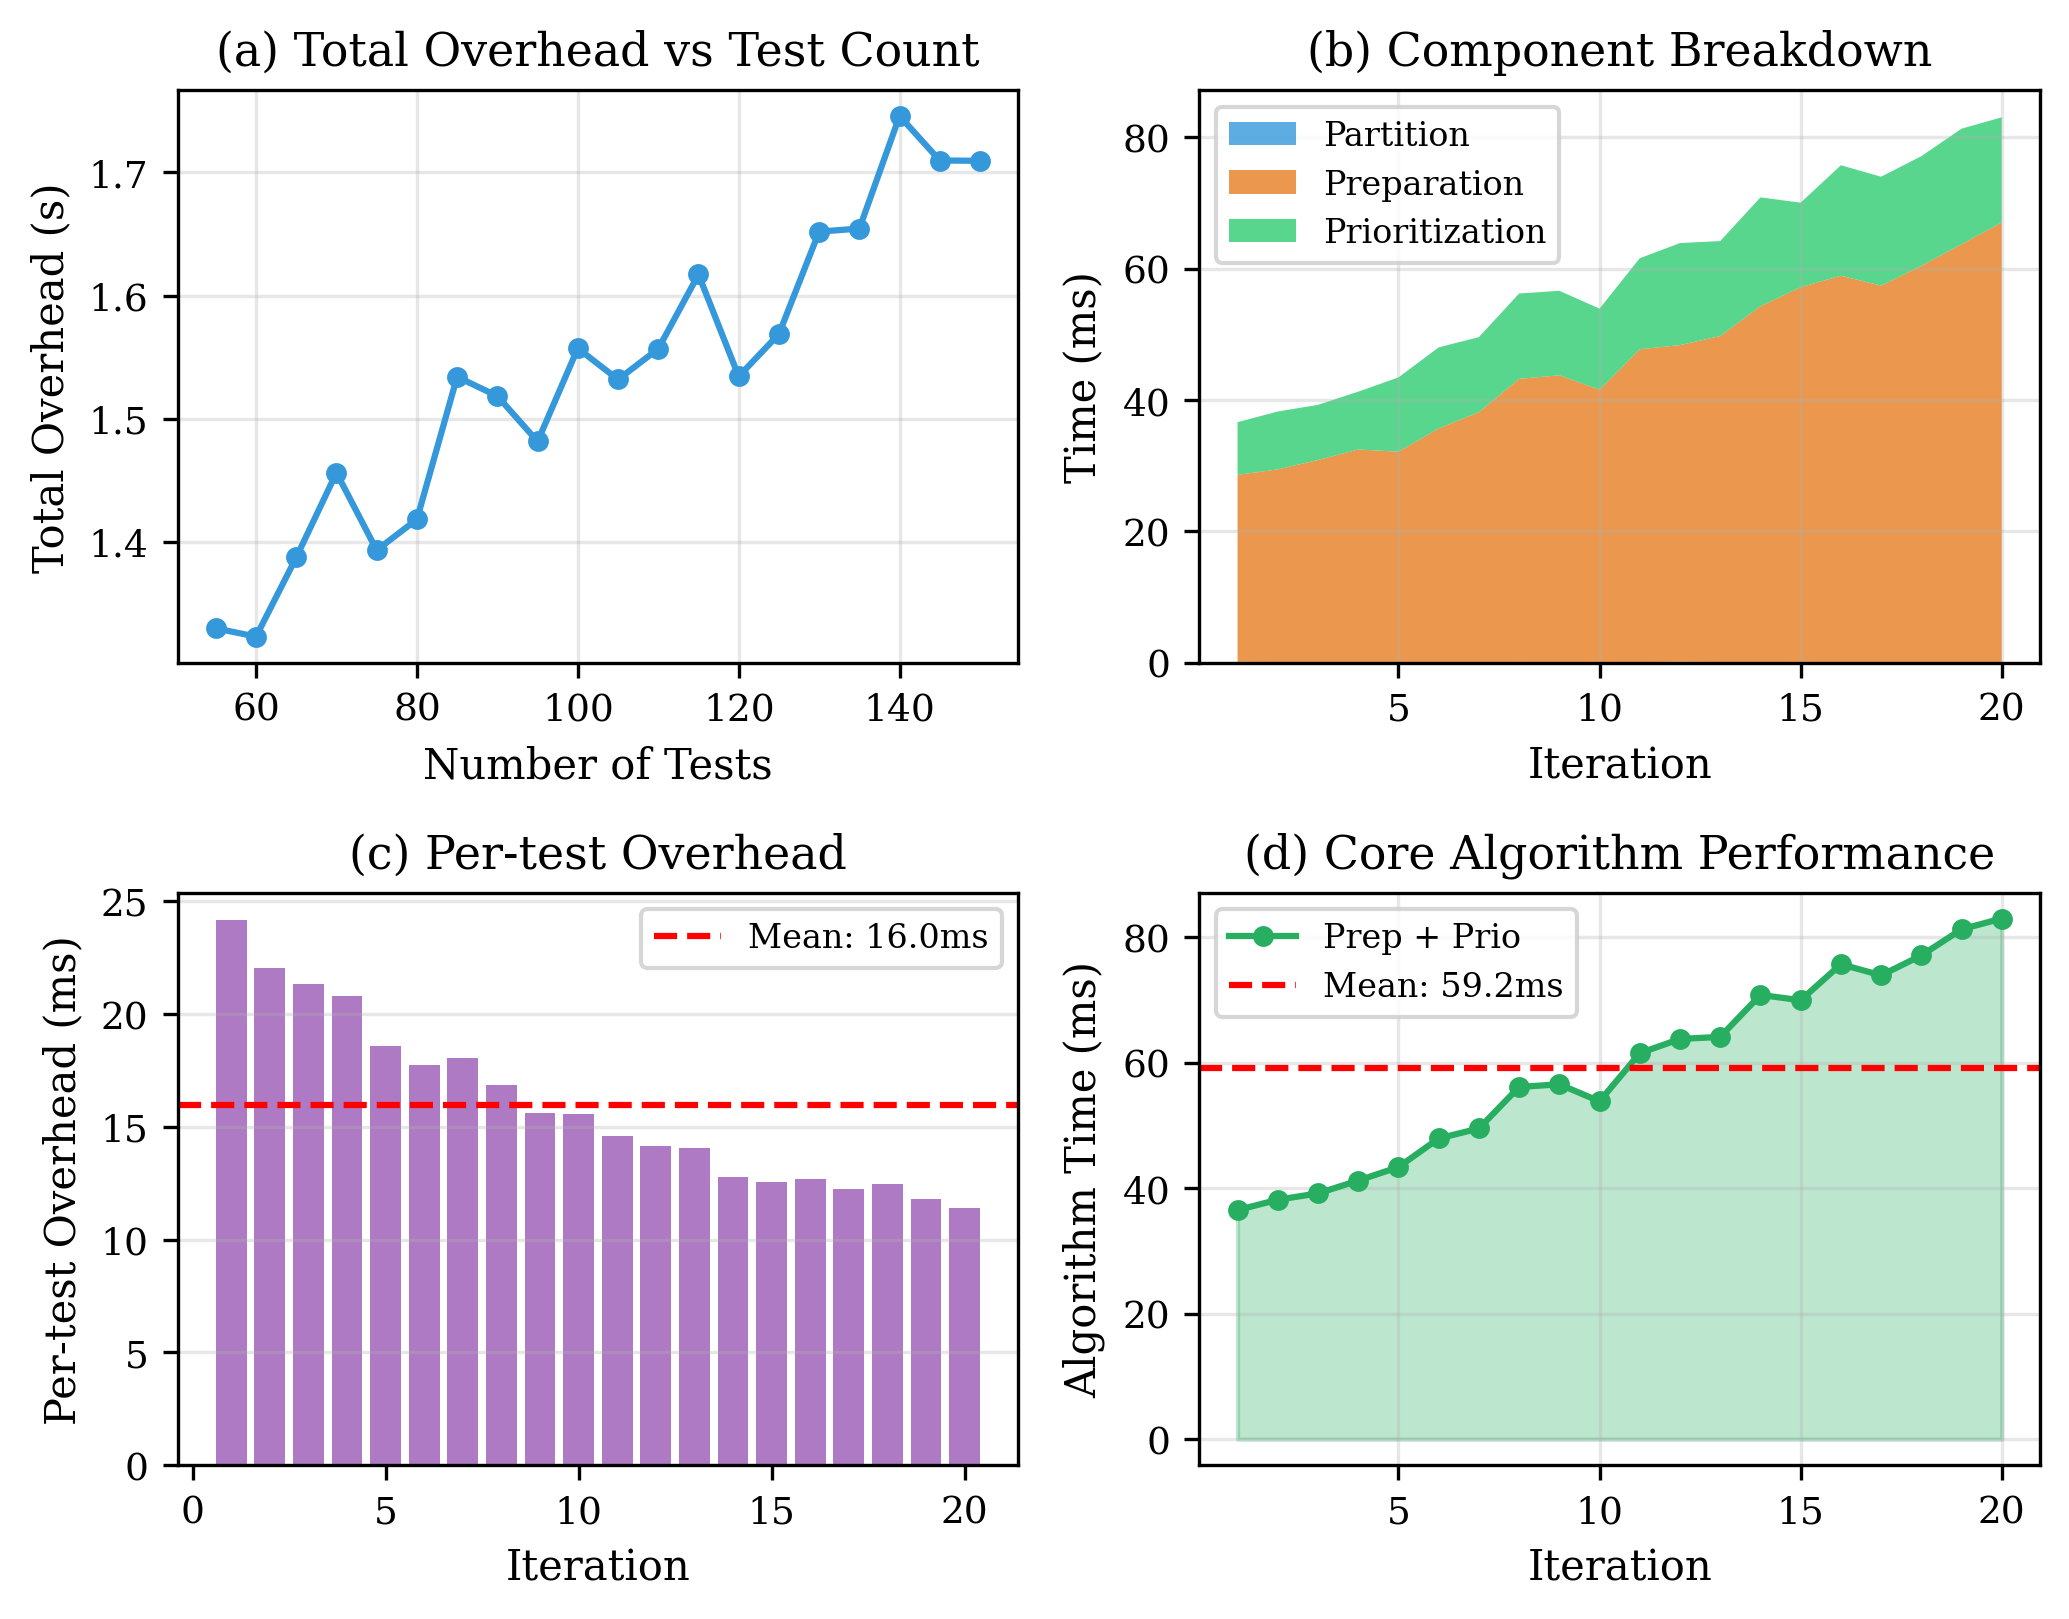
\includegraphics[width=0.86\linewidth]{figures/benchmark_grid.png}
\end{center}
\vspace{-0.08in}
{\fontsize{15}{18}\selectfont
\begin{tabular}{@{}lr@{}}
\toprule
Metric & Value \\
\midrule
Final synthetic suite size & 140 tests \\
Average total overhead & 1.51s \\
Average partition time & 0.1ms \\
Average preparation time & 29ms \\
Average prioritization time & 9ms \\
\bottomrule
\end{tabular}}
}

\posterblock{Takeaways}{
\begin{itemize}\tightitems
  \item fast-tcp packages FAST as a practical local tool with maintained framework integrations.
  \item Git-backed snapshots make repeated prioritization incremental.
  \item The core ranking step remains in the millisecond range; most cost is snapshot/preparation work.
  \item Future work: more frameworks, CI integrations, and coverage-aware white-box prioritization.
\end{itemize}

{\fontsize{14}{17}\selectfont
\textbf{Key reference:} B. Miranda, E. Cruciani, R. Verdecchia, and A. Bertolino. ``FAST approaches to scalable similarity-based test case prioritization.'' ICSE 2018.
}
}

\end{multicols}

\vfill
{\color{fastnavy}\rule{\linewidth}{4pt}}\par
{\fontsize{12}{15}\selectfont Poster distilled from \texttt{paper.tex}; designed as a visual aid with a single message, limited prose, and evidence-first figures.}

\end{document}
